\documentclass{article}
\usepackage{graphicx}
\begin{document}
\begin{titlepage}
	\centering
	\vfill
	\Huge{Primera práctica} \\
	\vfill
	\large{\textsc{Hugo Tonatiuh Carrillo Bonilla}}\\
	\vfill
	320026379
	\vfill
\end{titlepage}
\section*{Parte 1: Preparación del entorno.}
	Uso Fedora 44 :3
	\\
	\begin{figure}[h]
		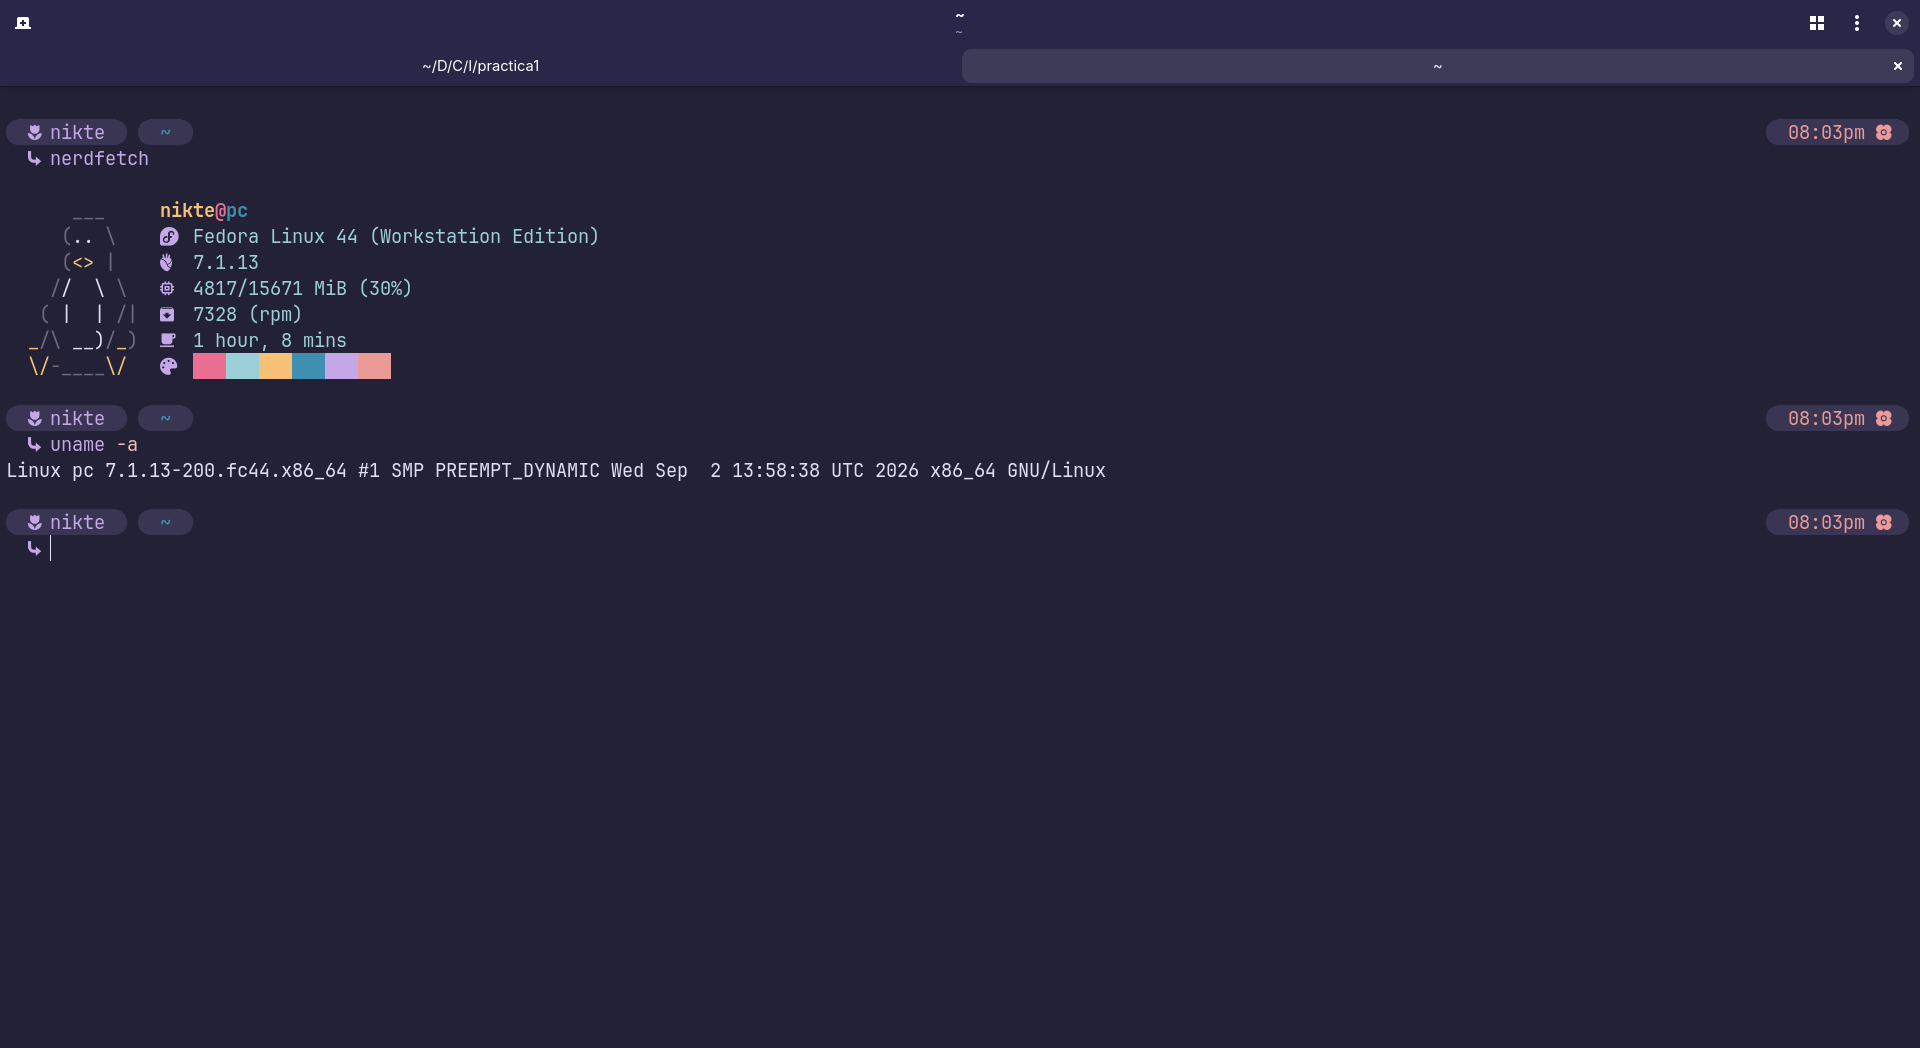
\includegraphics[width=\textwidth]{./images/capturaDos.png}
	\end{figure}
\section*{Parte 2: Uso de comandos básicos}
	\begin{enumerate}
		\item Usé los comandos \texttt{pwd} para saber en qué directorio estaba y \texttt{ls} para enlistar los archivos.
			\begin{center}
				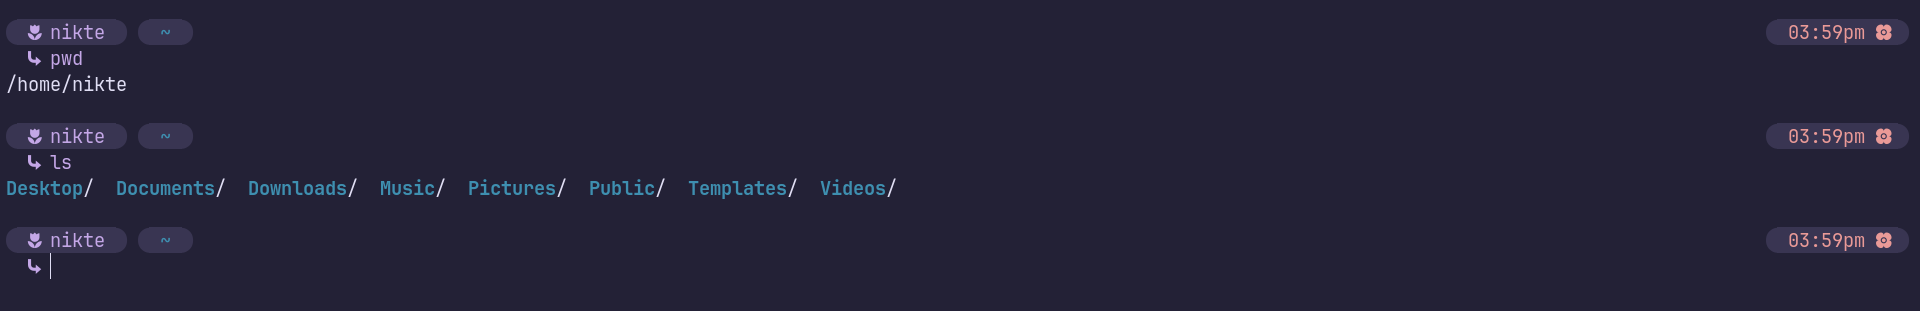
\includegraphics[width=\linewidth]{./images/Ej1.png}
			\end{center}
		\item Usé el comando \texttt{cd}.
			\begin{center}
				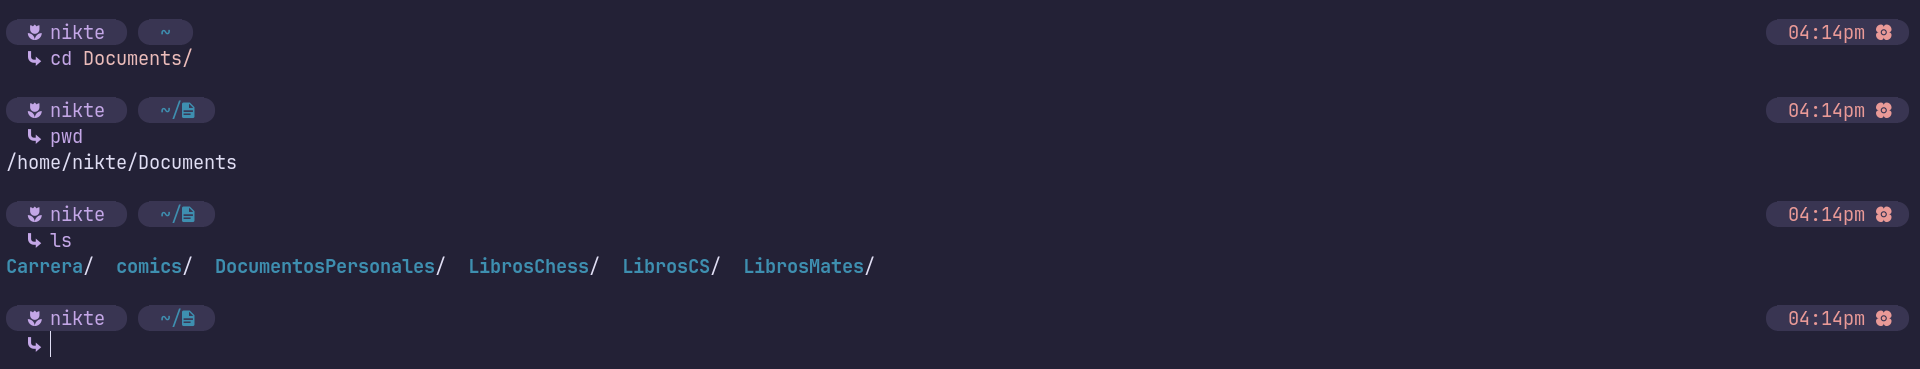
\includegraphics[width=\linewidth]{./images/Ej2.png}
			\end{center}
		\item Usé el comando \texttt{mkdir -p} para no tener que usar el mismo comando muchas veces y después usé \texttt{tree} para verificar que la jerarquía era la correcta.
			\begin{center}
				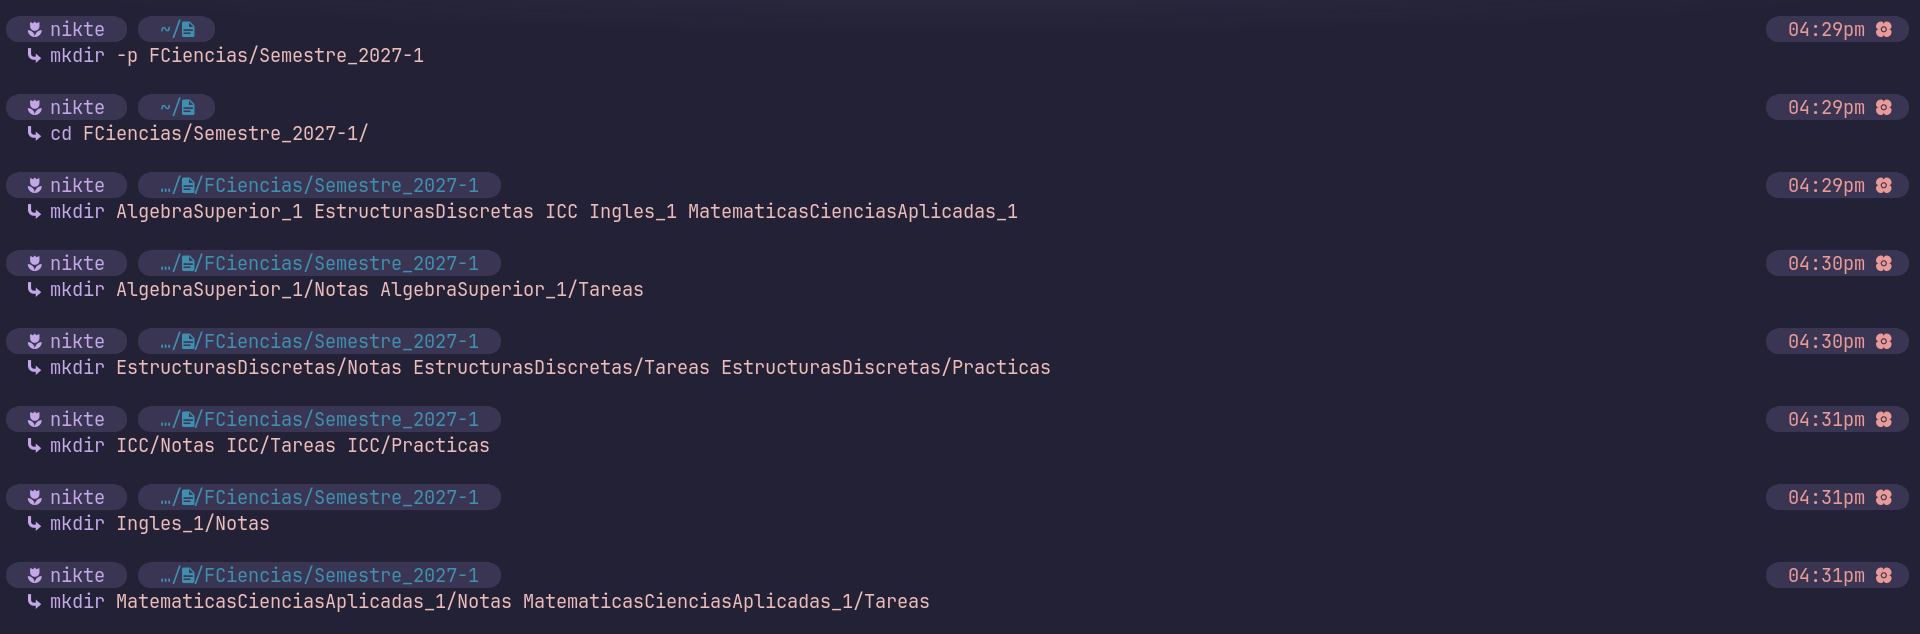
\includegraphics[width=\linewidth]{./images/Ej3-1.png}\\
				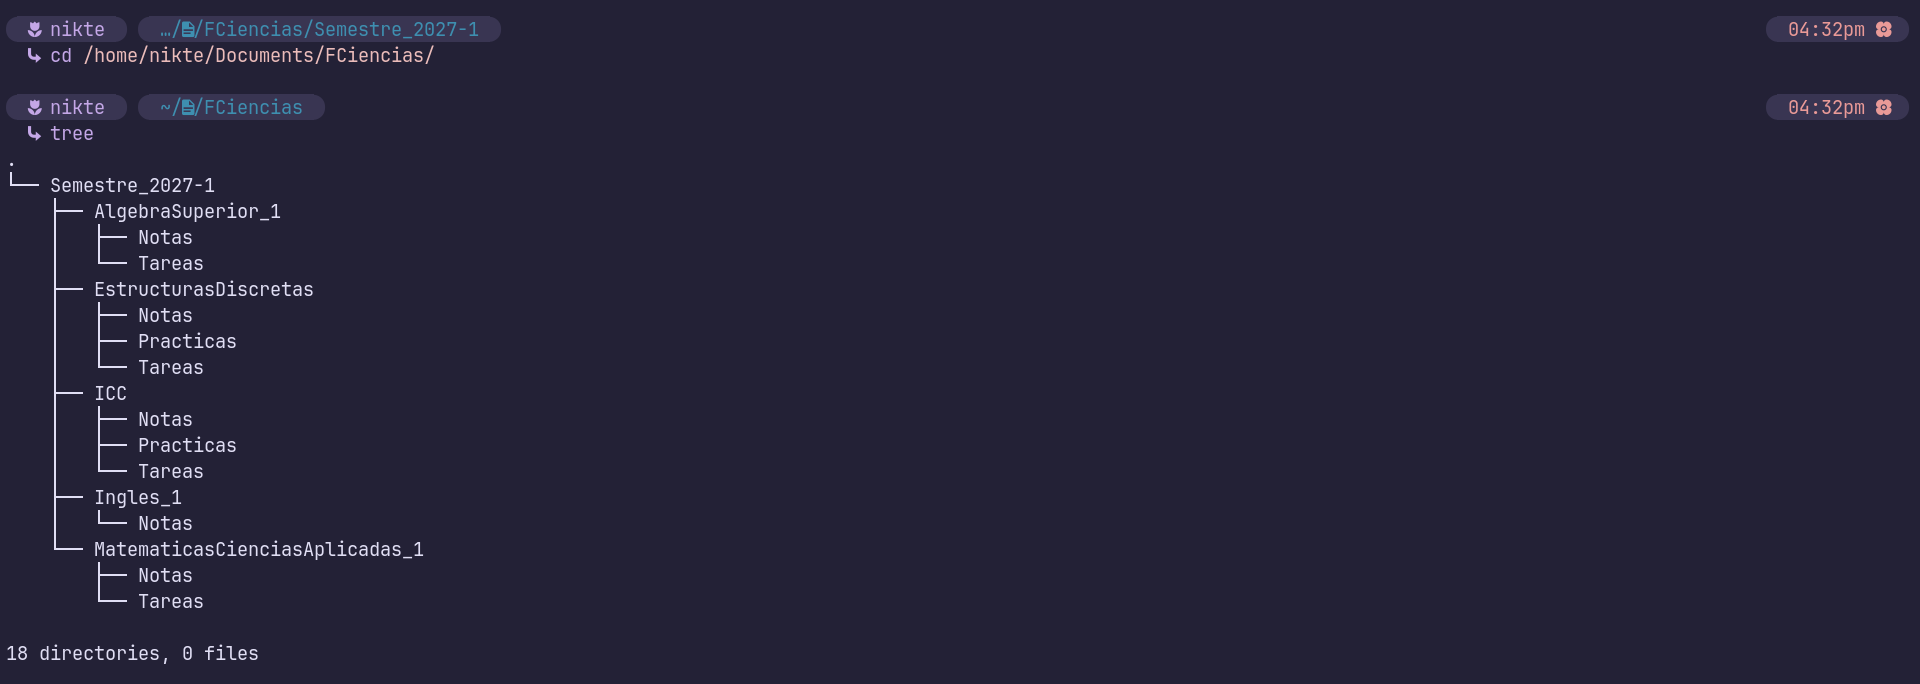
\includegraphics[width=\linewidth]{./images/Ej3-2.png}\\
			\end{center}
		\item Utilicé \textit{neovim} (\texttt{nvim})para crear y editar el archivo. Después utilicé \texttt{cat} para mostrar sus contenidos.
			\begin{center}
				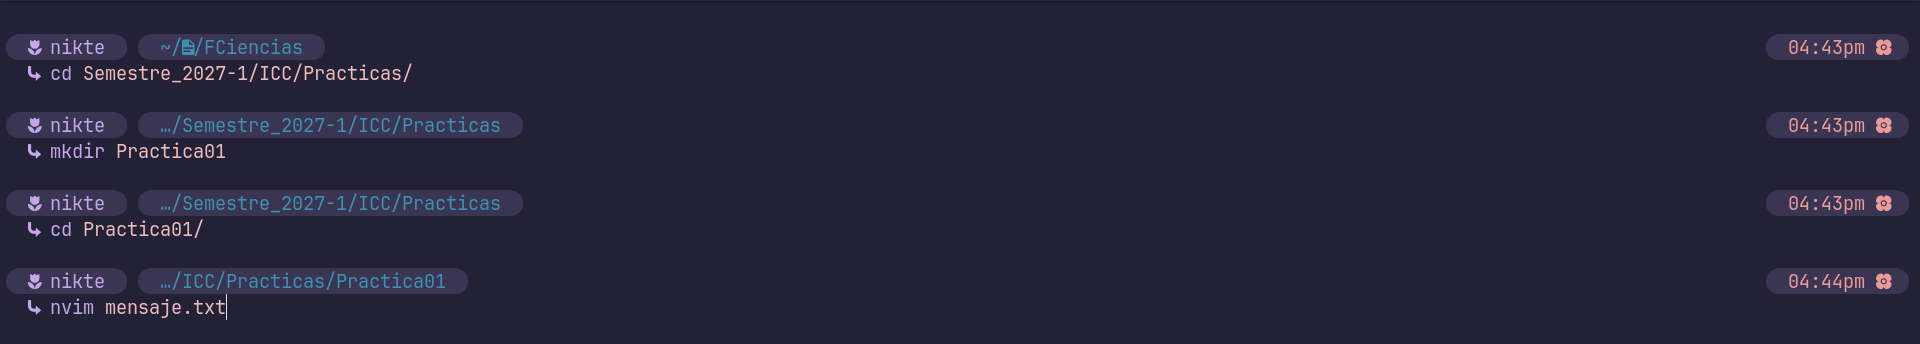
\includegraphics[width=\linewidth]{./images/Ej4-1.png}\\
				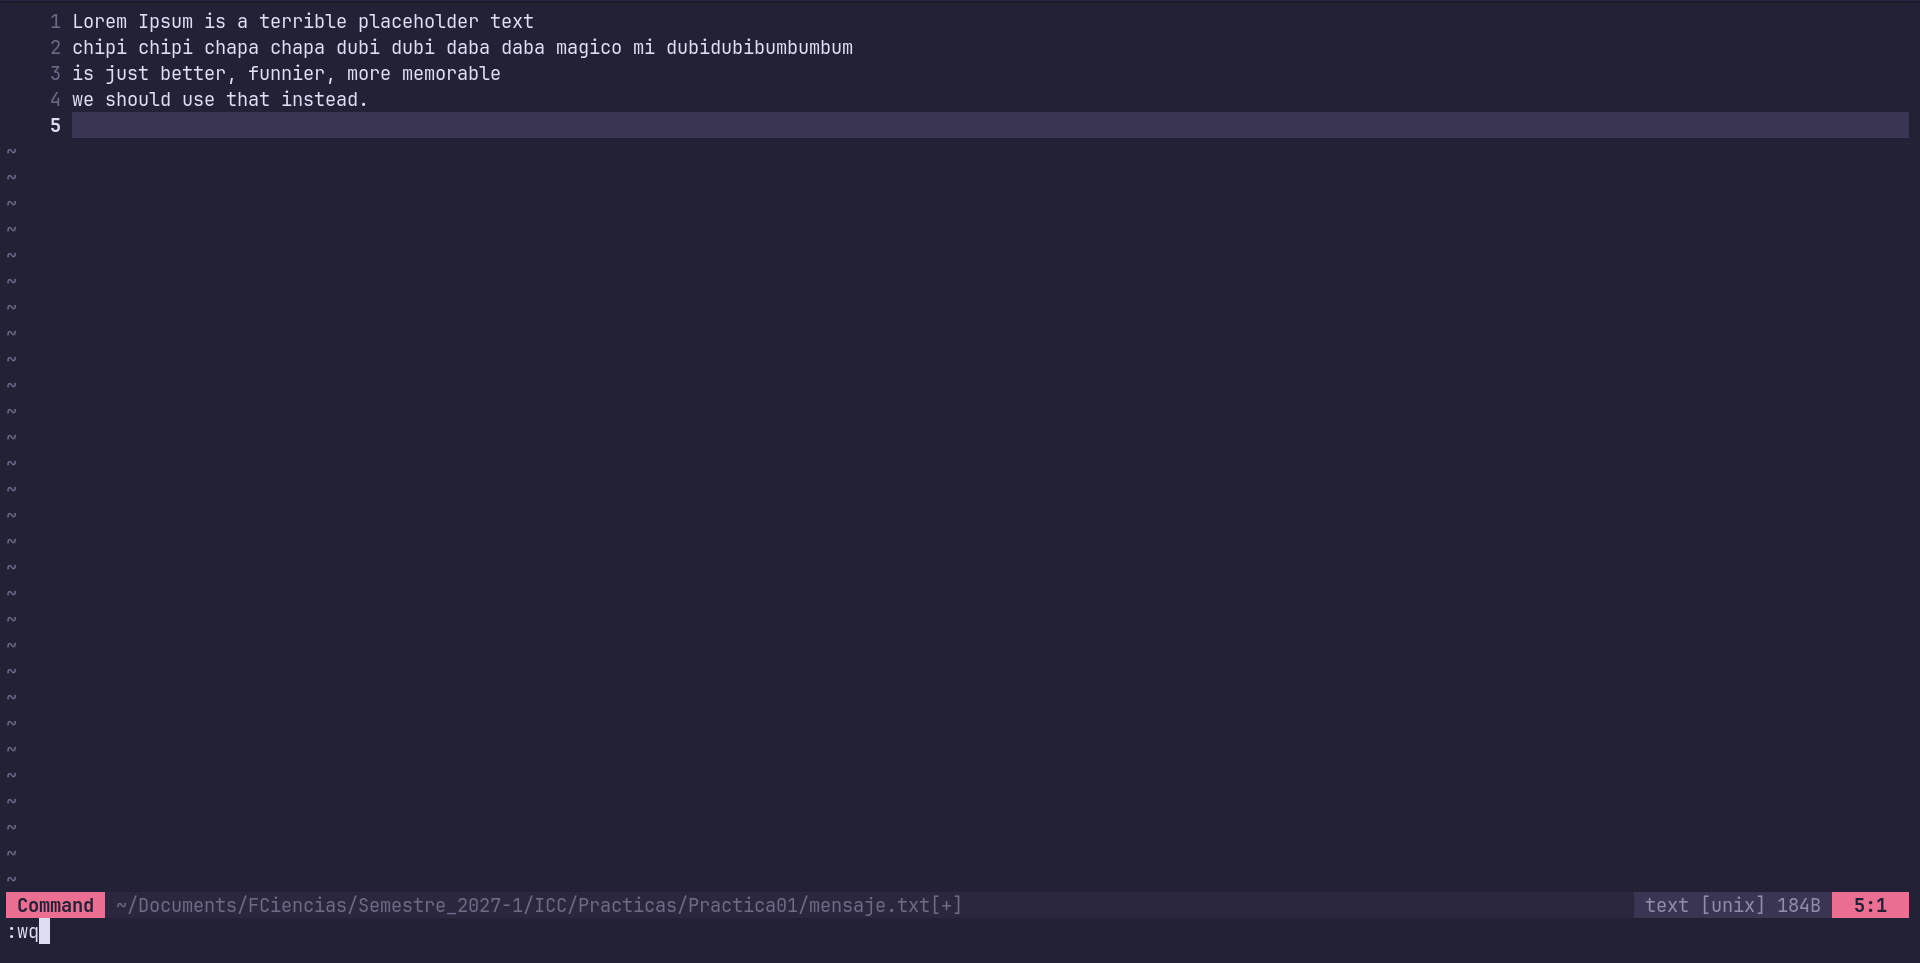
\includegraphics[width=\linewidth]{./images/Ej4-2.png}\\
				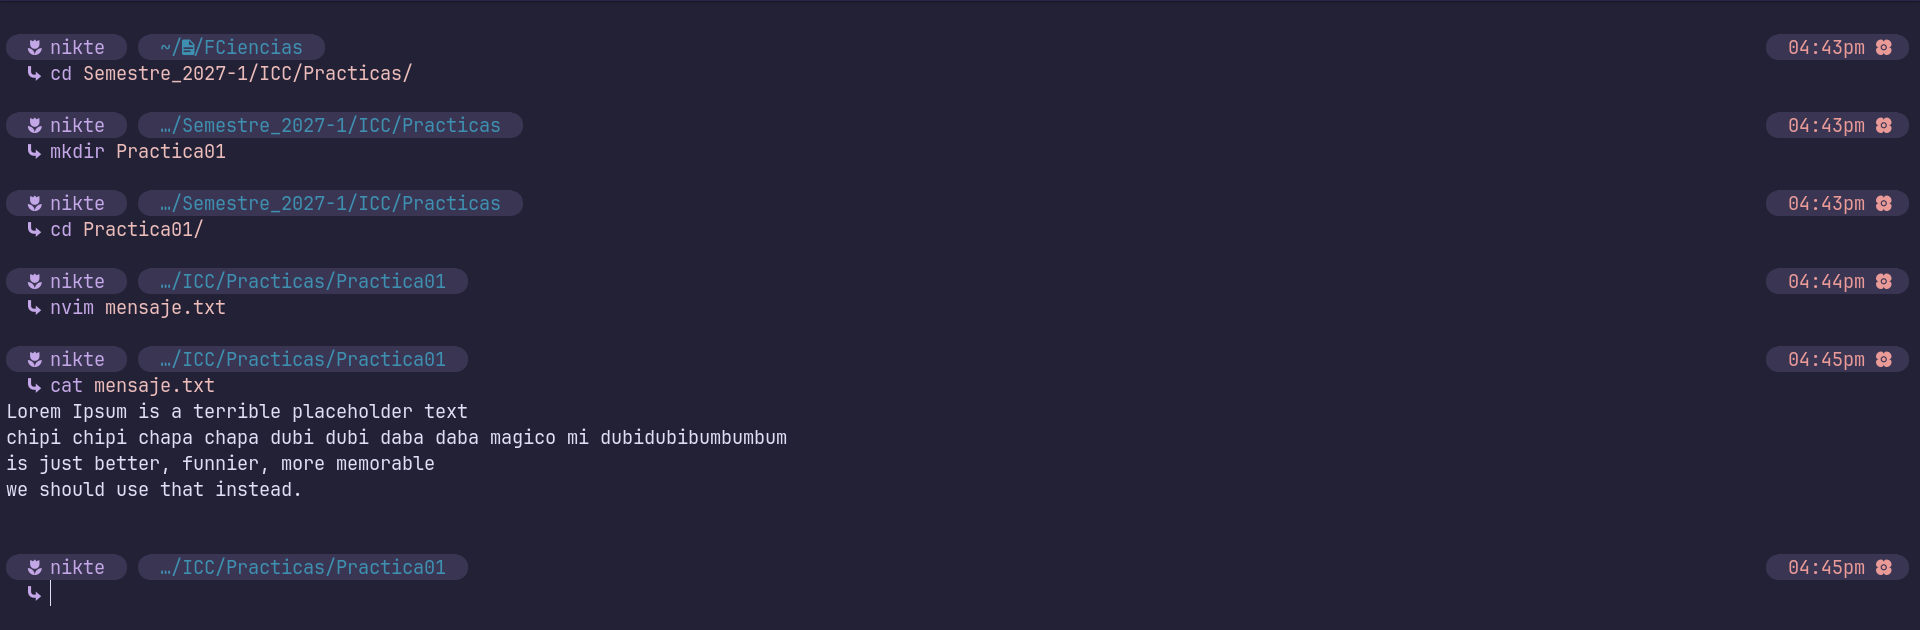
\includegraphics[width=\linewidth]{./images/Ej4-3.png}\\
			\end{center}
		\item Usé \texttt{cp} y \texttt{mv} para copiar y mover los archivos.
			\begin{center}
				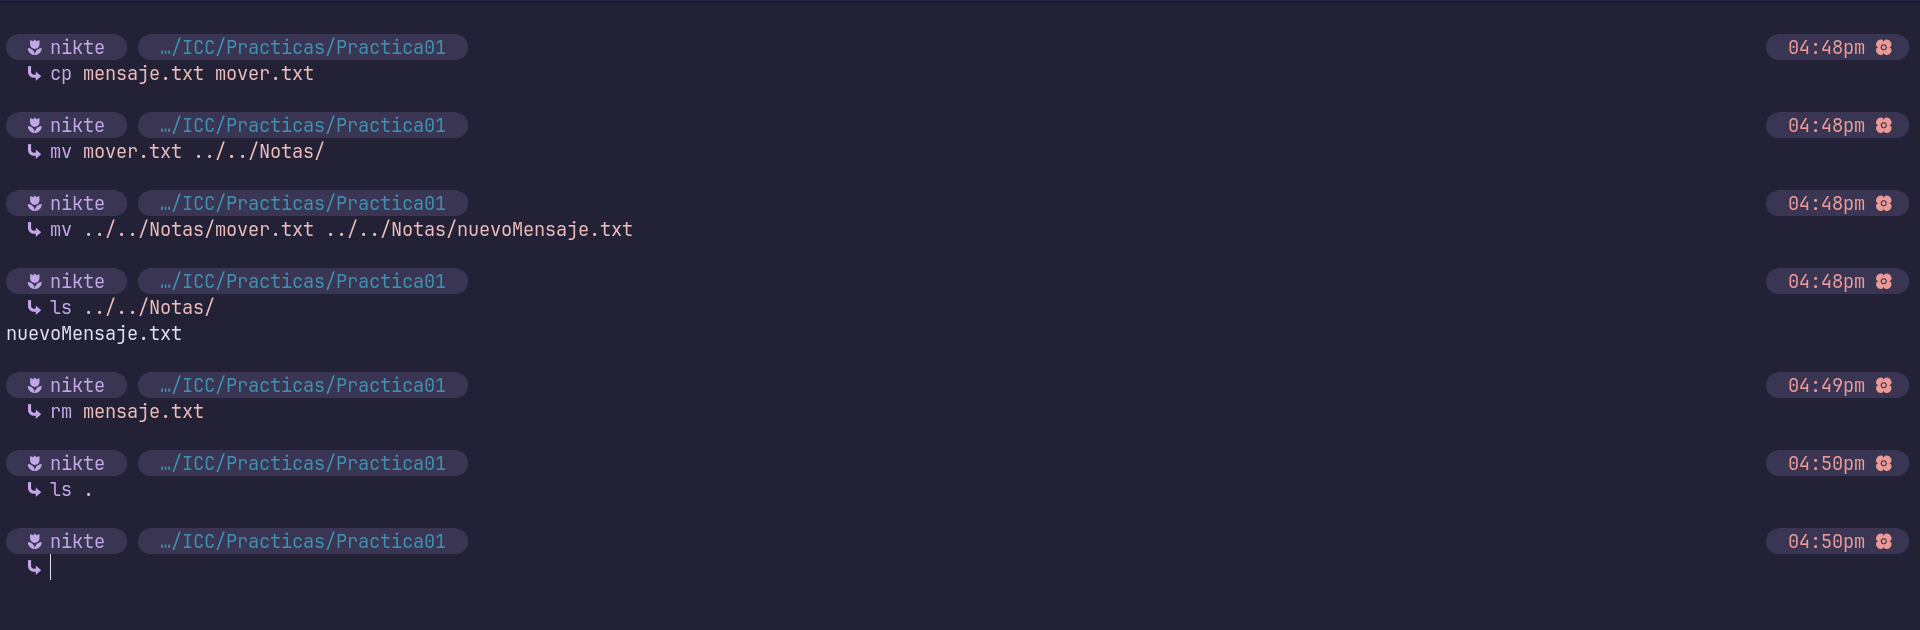
\includegraphics[width=\linewidth]{./images/Ej-5.png}
			\end{center}
		\item Los comandos que investigué son:
			\begin{itemize}
				\item \texttt{ip} Sirve para mostrar o manipular dispositivos, interfaces y túneles de networking.
				\item \texttt{fold} Inserta saltos de línea en archivos (o input) para que tengan una longitud de línea consistente.
				\item \texttt{awk} Es un lenguaje que sirve para procesar texto y es tan poderoso que podría hacer 6 ejercicios nada más de este comando.
				\item \texttt{tsort} A lxs computólogxs les encanta ordenar, es como la mitad de la carrera y obviamente iban a tener un programa nada más para eso.
				\item \texttt{nc} Sirve para leer y escribir datos a través del protocolo TCP/IP.
			\end{itemize}
			\textbf{Ejercicio:} Extrae todas las interfaces IP activas con \texttt{ip}, y con \texttt{nc} asígnales un listener que no haga nada. Con \texttt{awk} extrae de las direcciones IP todos los dígitos separados por un punto, ponlos en un array y ordénalo con \texttt{tsort}. Finalmente, toma el mayor de esos valores y trunca el límite de longitud de líneas de \texttt{mensaje.txt} con \texttt{fold}. \\
			\\
			Hice el ejercicio pero tuve que usar un comando aparte de los cinco que había investigado. Además, por razones de seguridad tengo que bloquear ciertas partes de la imagen.
			\begin{center}
				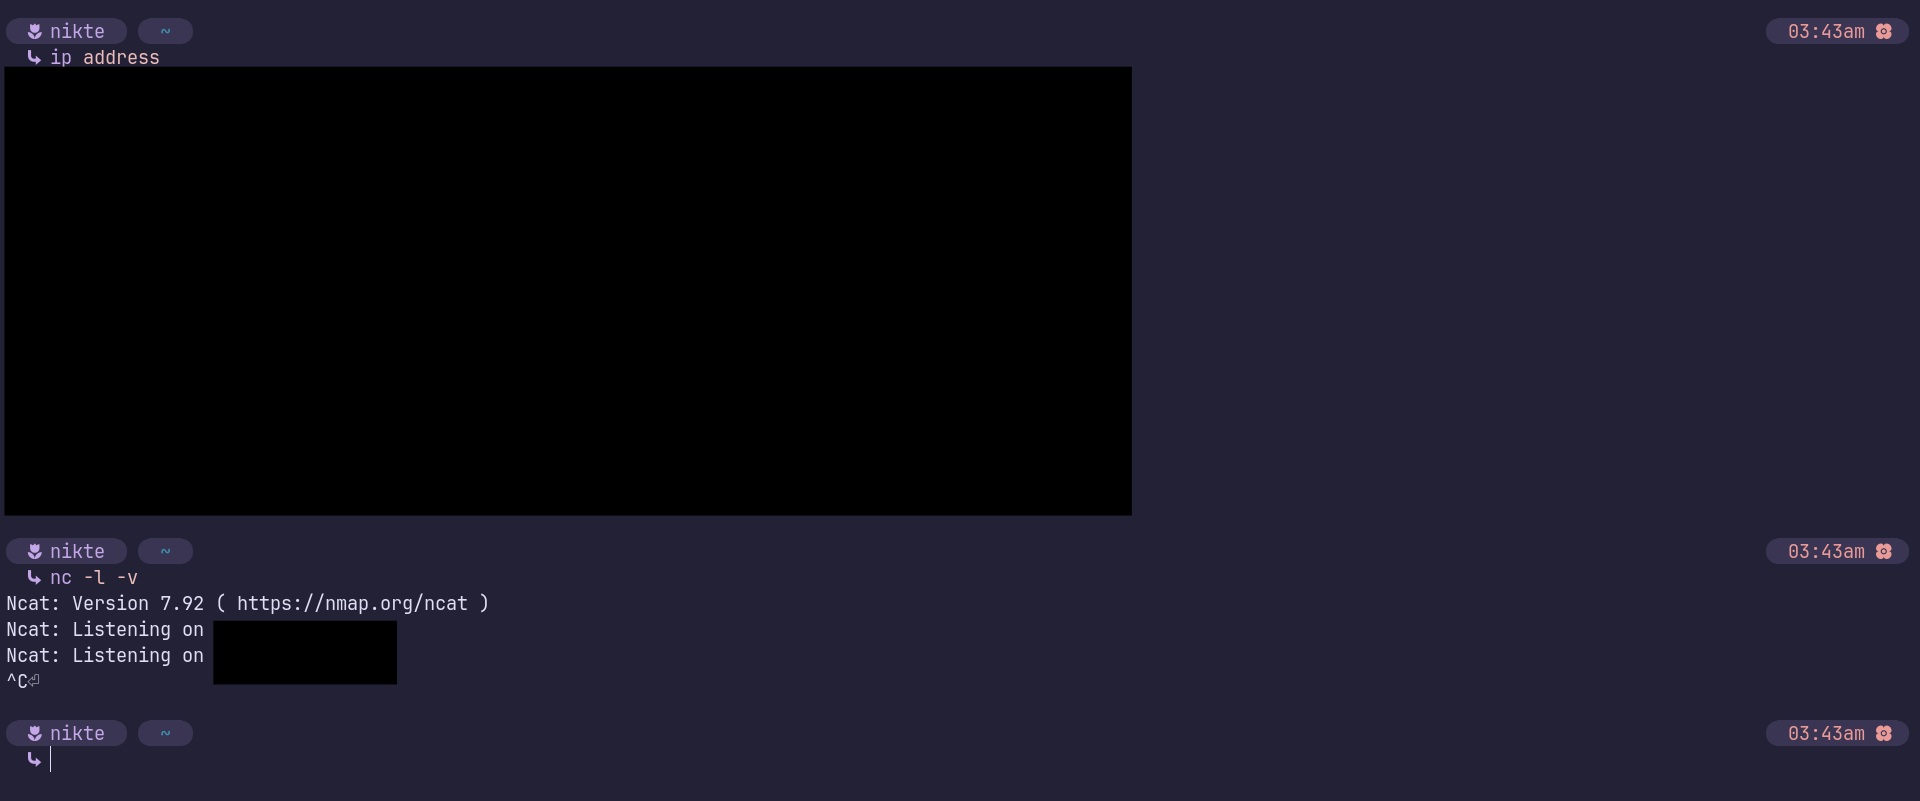
\includegraphics[width=\linewidth]{./images/Ej6-1.png}\\
				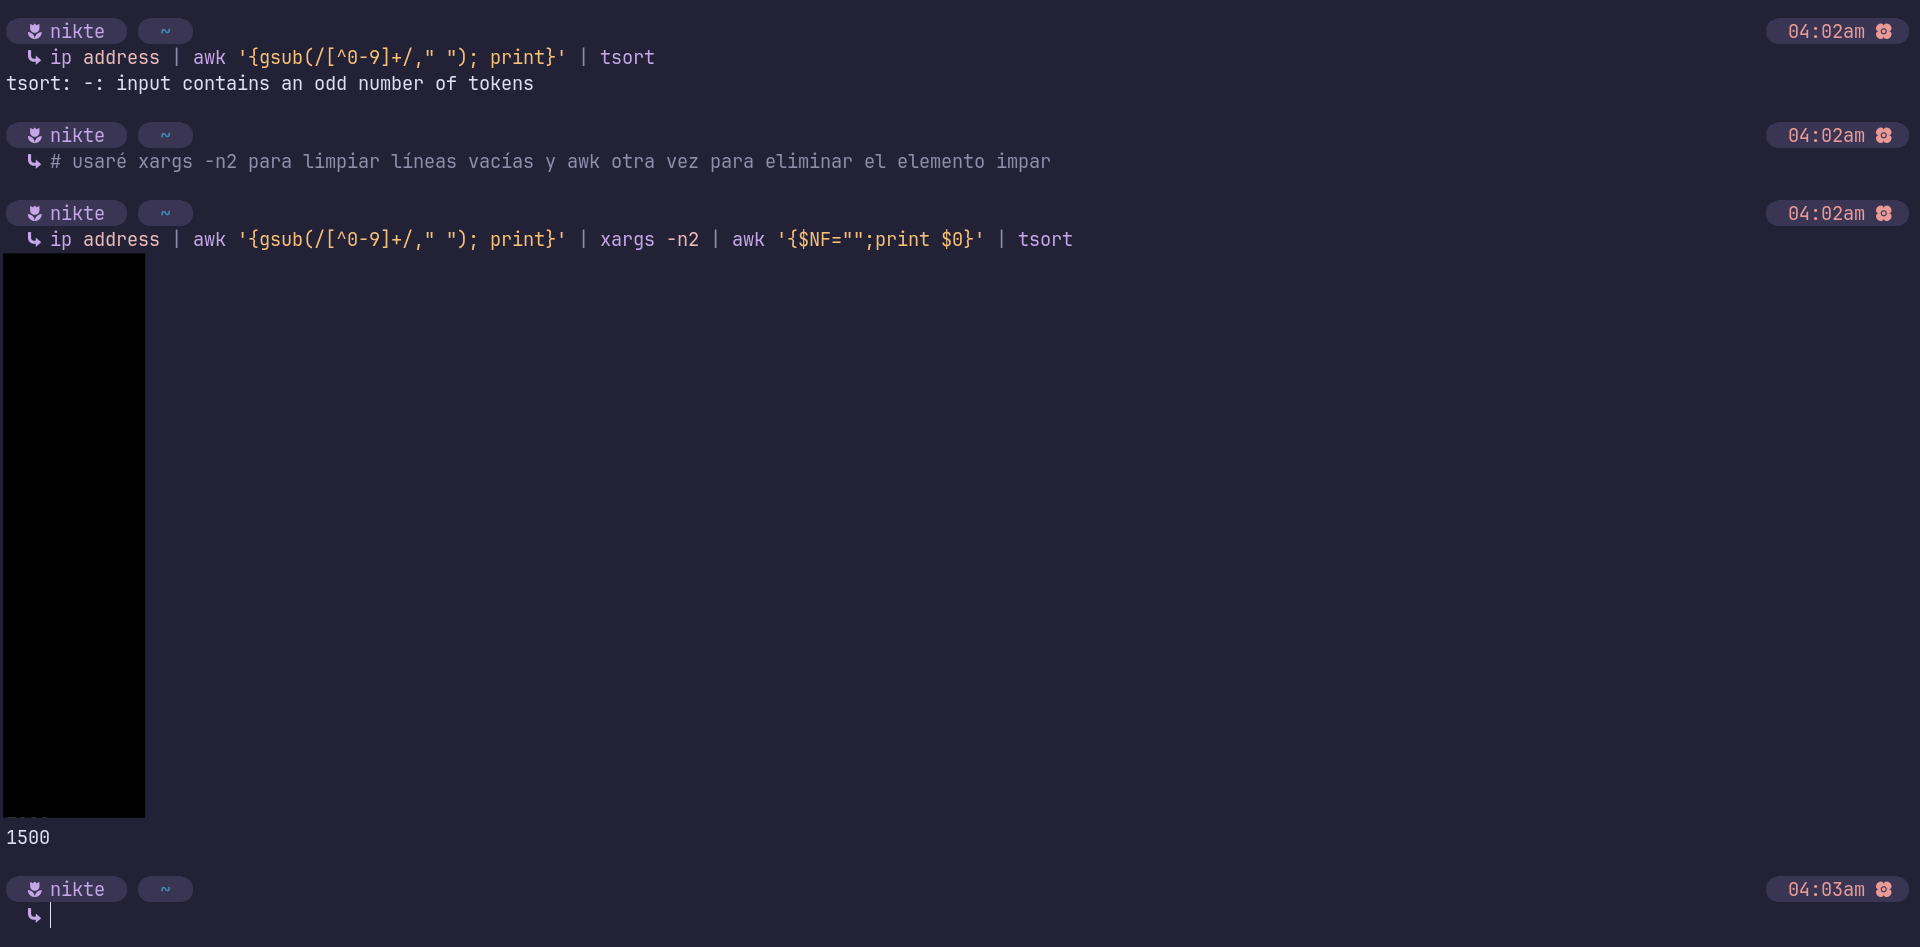
\includegraphics[width=\linewidth]{./images/Ej6-2.png}\\
				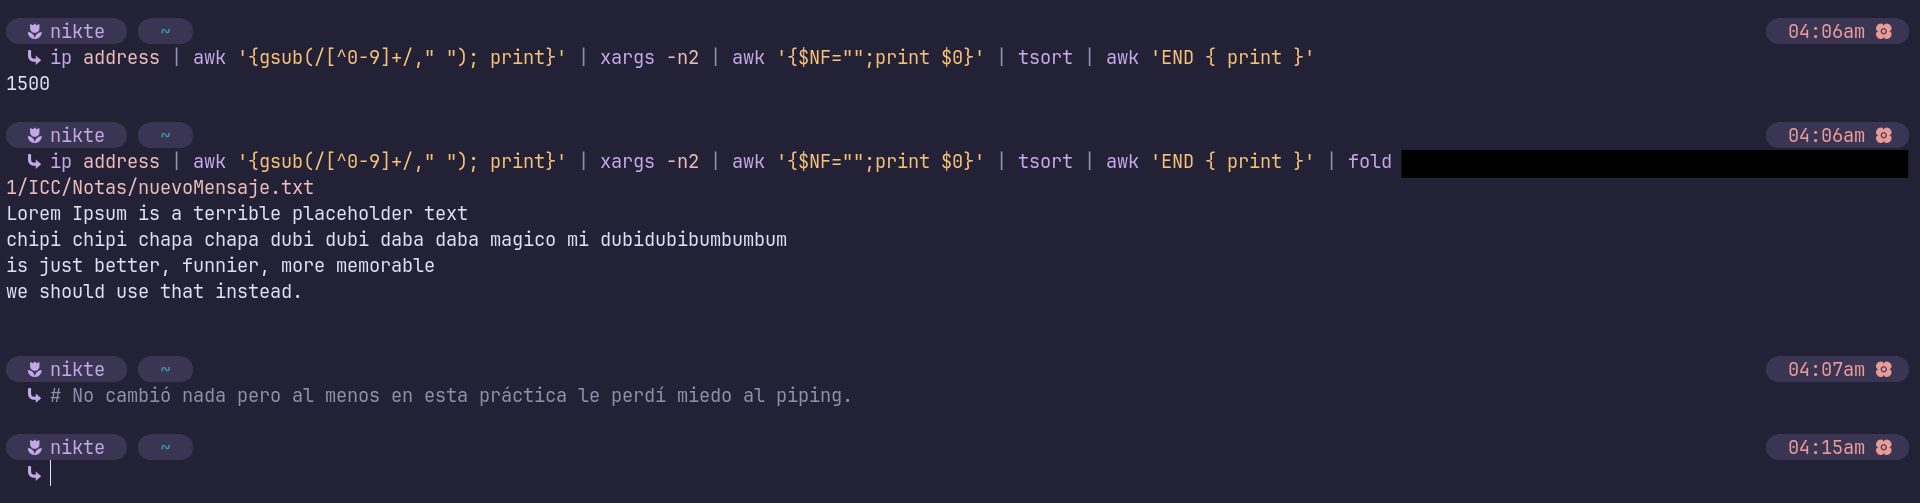
\includegraphics[width=\linewidth]{./images/Ej6-3.png}\\
			\end{center}
	\end{enumerate}
\section*{Parte 3: Instalación de JDK}
	\begin{center}
		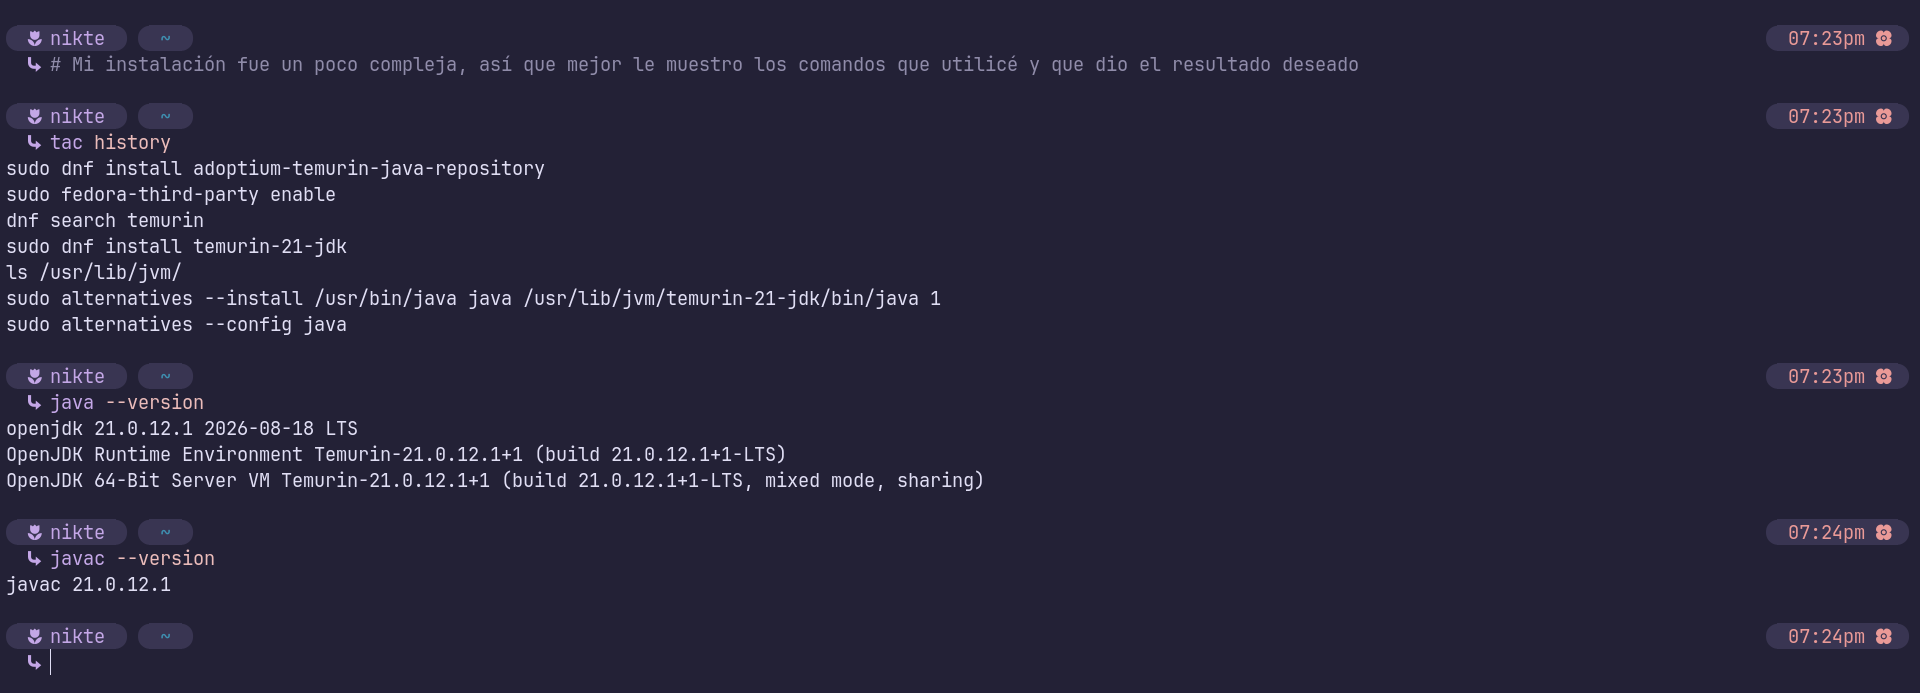
\includegraphics[width=\linewidth]{./images/java.png}
	\end{center}
\section*{Conclusión}
En esta práctica aprendimos a movernos entre archivos, hacer cambios mínimos y realizar operaciones triviales en los sistemas adyacentes a UNIX. También vimos cómo podemos componer estos comandos sencillos a través del piping y descubrimos que podemos leer y escribir a archivos con nuestros comandos de la terminal. En lo personal, nunca había utilizado más de un pipe en mi vida y me alegra haber logrado una tarea que normalmente hubiera realizado con un script de Python. Es un primer paso hacia destapar nuestro potencial como desarrolladorxs.
\end{document}
